\documentclass{beamer}
\usetheme{metropolis}

\usepackage[spanish]{babel}
\usepackage[utf8]{inputenc}
\usepackage{tikz}
\usepackage{xcolor}
\usepackage{amsmath}
\usepackage{listings}

% Definición de colores personalizados
\definecolor{primary}{RGB}{46, 204, 113}
\definecolor{secondary}{RGB}{52, 152, 219}
\definecolor{accent}{RGB}{231, 76, 60}
\definecolor{background}{RGB}{236, 240, 241}
\definecolor{gradient1}{RGB}{255, 107, 107}
\definecolor{gradient2}{RGB}{255, 159, 67}

% Configuración del tema
\setbeamercolor{normal text}{fg=black,bg=background}
\setbeamercolor{structure}{fg=primary}
\setbeamercolor{alerted text}{fg=accent}

\definecolor{lightgray}{rgb}{0.95,0.95,0.95}
\definecolor{darkgreen}{rgb}{0,0.5,0}
\definecolor{darkblue}{rgb}{0,0,0.5}

\lstset{
  backgroundcolor=\color{lightgray},
  basicstyle=\tiny\ttfamily,
  keywordstyle=\color{darkblue}\bfseries,
  commentstyle=\color{darkgreen},
  stringstyle=\color{red},
  numbers=left,
  numberstyle=\tiny\color{gray},
  stepnumber=1,
  numbersep=5pt,
  showspaces=false,
  showstringspaces=false,
  showtabs=false,
  frame=single,
  tabsize=2,
  language=Python,
  breaklines=true,
  breakatwhitespace=true
}

\title{\Huge\textbf{Validación de Modelos}}
\author{Analítica de Datos, Universidad de San Andrés}
\date{}

\begin{document}

\begin{frame}
    \titlepage
\end{frame}

\begin{frame}{Matriz de Confusión Binaria}
    \begin{center}
    \begin{tikzpicture}[scale=0.8]
    \draw (0,0) rectangle (4,4);
    \draw (0,2) -- (4,2);
    \draw (2,0) -- (2,4);
    
    \node[above] at (2,4) {\textbf{Real}};
    \node[left] at (0,2) {\textbf{Predicho}};
    
    \fill[green!30] (0,2) rectangle (2,4);
    \fill[red!30] (2,0) rectangle (4,2);
    \fill[blue!30] (0,0) rectangle (2,2);
    \fill[yellow!30] (2,2) rectangle (4,4);
    
    \node at (1,3) {VP};
    \node at (3,3) {FP};
    \node at (1,1) {FN};
    \node at (3,1) {VN};
    \end{tikzpicture}
    \hspace{0.5cm}
    \begin{tikzpicture}[scale=0.8]
    \draw (0,0) rectangle (4,4);
    \draw (0,2) -- (4,2);
    \draw (2,0) -- (2,4);
    
    \node[above] at (2,4) {\textbf{Predicho}};
    \node[left] at (0,2) {\textbf{Real}};
    
    \fill[green!30] (0,2) rectangle (2,4);
    \fill[red!30] (2,0) rectangle (4,2);
    \fill[yellow!30] (0,0) rectangle (2,2);
    \fill[blue!30] (2,2) rectangle (4,4);
    
    \node at (1,3) {VP};
    \node at (3,3) {FN};
    \node at (1,1) {FP};
    \node at (3,1) {VN};
    \end{tikzpicture}
    \end{center}
    
    \begin{itemize}
        \item VP: Verdaderos Positivos
        \item VN: Verdaderos Negativos
        \item FP: Falsos Positivos
        \item FN: Falsos Negativos
    \end{itemize}
\end{frame}

\begin{frame}{Matriz de Confusión Multiclase}
    \begin{center}
    \begin{tikzpicture}[scale=0.7]
    \node[above] at (3,7) {\textbf{R}};
    \node[left] at (-1,3) {\textbf{P}};
    
    \draw (0,0) rectangle (6,6);
    \draw (0,2) -- (6,2);
    \draw (0,4) -- (6,4);
    \draw (2,0) -- (2,6);
    \draw (4,0) -- (4,6);
    
    \fill[green!30] (0,4) rectangle (2,6);
    \fill[green!30] (2,2) rectangle (4,4);
    \fill[green!30] (4,0) rectangle (6,2);
    
    \node at (1,5) {85};
    \node at (3,5) {10};
    \node at (5,5) {5};
    \node at (1,3) {8};
    \node at (3,3) {82};
    \node at (5,3) {10};
    \node at (1,1) {7};
    \node at (3,1) {12};
    \node at (5,1) {81};
    
    \node at (-0.5,5) {L};
    \node at (-0.5,3) {N};
    \node at (-0.5,1) {S};
    
    \node at (1,6.5) {L};
    \node at (3,6.5) {N};
    \node at (5,6.5) {S};
    \end{tikzpicture}
    \end{center}
    
    \begin{itemize}
        \item L: Lluvia
        \item N: Nublado
        \item S: Soleado
    \end{itemize}
\end{frame}

\begin{frame}{Accuracy (Exactitud)}
    \begin{center}
    \Large Accuracy = $\frac{\colorbox{green!30}{VP} + \colorbox{red!30}{VN}}{\colorbox{green!30}{VP} + \colorbox{red!30}{VN} + \colorbox{yellow!30}{FP} + \colorbox{blue!30}{FN}}$
    \end{center}
    Es el porcentaje total de predicciones correctas que hace nuestro modelo.
\end{frame}

\begin{frame}{Precision (Precisión)}
    \begin{center}
    \Large Precision = $\frac{\colorbox{green!30}{VP}}{\colorbox{green!30}{VP} + \colorbox{yellow!30}{FP}}$
    \end{center}
    Es qué tan confiables son nuestras predicciones positivas.
\end{frame}

\begin{frame}{Specificity (Especificidad) / True Negative Rate (TNR)}
    \begin{center}
    \Large Specificity = $\frac{\colorbox{red!30}{VN}}{\colorbox{red!30}{VN} + \colorbox{yellow!30}{FP}}$
    \end{center}
    Es qué tan bien identificamos los casos negativos correctamente.
\end{frame}

\begin{frame}{Recall (Sensibilidad) / True Positive Rate (TPR)}
    \begin{center}
    \Large Recall (TPR) = $\frac{\colorbox{green!30}{VP}}{\colorbox{green!30}{VP} + \colorbox{blue!30}{FN}}$
    \end{center}
    Es qué tan bien detectamos todos los casos positivos que existen.
\end{frame}

\begin{frame}{Fall-out / False Positive Rate (FPR)}
    \begin{center}
    \Large Fall-out (FPR) = $\frac{\colorbox{yellow!30}{FP}}{\colorbox{yellow!30}{FP} + \colorbox{red!30}{VN}}$
    \end{center}
    Es qué tan seguido nos equivocamos prediciendo casos positivos.
\end{frame}

\begin{frame}{Miss Rate / False Negative Rate (FNR)}
    \begin{center}
    \Large Miss Rate (FNR) = $\frac{\colorbox{blue!30}{FN}}{\colorbox{blue!30}{FN} + \colorbox{green!30}{VP}}$
    \end{center}
    Es qué tan seguido nos perdemos casos positivos que deberíamos haber detectado.
\end{frame}

\begin{frame}{F1-Score}
    \begin{center}
    \Large F1-Score = $2 \times \frac{Precision \times Recall}{Precision + Recall}$
    \end{center}
    Es un balance entre la precisión y el recall, útil cuando las clases están desbalanceadas.
\end{frame}

\begin{frame}{False Discovery Rate (FDR)}
    \begin{center}
    \Large FDR = $\frac{\colorbox{yellow!30}{FP}}{\colorbox{yellow!30}{FP} + \colorbox{green!30}{VP}}$
    \end{center}
    Es qué tan seguido nos equivocamos cuando hacemos predicciones positivas.
\end{frame}

\begin{frame}{False Omission Rate (FOR)}
    \begin{center}
    \Large FOR = $\frac{\colorbox{blue!30}{FN}}{\colorbox{blue!30}{FN} + \colorbox{red!30}{VN}}$
    \end{center}
    Es qué tan seguido nos equivocamos cuando hacemos predicciones negativas.
\end{frame}

\begin{frame}{Negative Predictive Value (NPV)}
    \begin{center}
    \Large NPV = $\frac{\colorbox{red!30}{VN}}{\colorbox{red!30}{VN} + \colorbox{blue!30}{FN}}$
    \end{center}
    Es qué tan confiables son nuestras predicciones negativas.
\end{frame}

\begin{frame}{Curva ROC}
    \begin{center}
    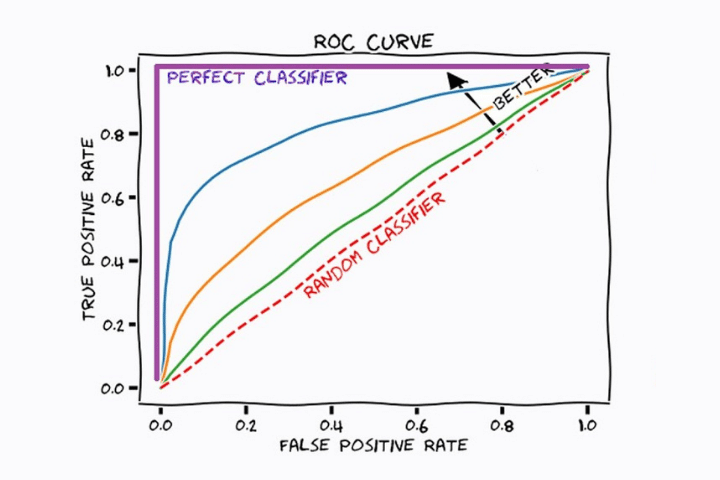
\includegraphics[width=0.7\textwidth]{curva-roc.png}
    \end{center}

    La curva ROC muestra la relación entre TPR y FPR para diferentes umbrales. El área bajo la curva (AUC) indica el rendimiento del modelo.
\end{frame}

\begin{frame}{¿Cómo entender la curva ROC?}

    Para cada punto de umbral existe una tasa de falsos positivos y una tasa de verdaderos positivos. Las coordenadas que trazamos son (FPR, TPR) en el eje X e Y respectivamente. Recordamos que:

    \vspace{1em}

    \begin{center}
    Fall-out (FPR) = $\frac{\colorbox{yellow!30}{FP}}{\colorbox{yellow!30}{FP} + \colorbox{red!30}{VN}}$

    Recall (TPR) = $\frac{\colorbox{green!30}{VP}}{\colorbox{green!30}{VP} + \colorbox{blue!30}{FN}}$
    \end{center}
\end{frame}

\begin{frame}{Umbral 0 - Clasificar todo como positivo (1/2)}
    En el caso de un umbral 0, todo esta siendo calificado como positivo porque esta a la derecha del umbral, entonces:

    \begin{center}
    \begin{tikzpicture}
    \draw (0,0) rectangle (4,4);
    \draw (0,2) -- (4,2);
    \draw (2,0) -- (2,4);
    
    \node[above] at (2,4) {\textbf{R}};  
    \node[left] at (0,2) {\textbf{P}};
    
    \fill[green!30] (0,2) rectangle (2,4);
    \fill[red!30] (2,0) rectangle (4,2);
    \fill[blue!30] (0,0) rectangle (2,2);
    \fill[yellow!30] (2,2) rectangle (4,4);
    
    \node at (1,3) {$\alpha$ (VP)};
    \node at (3,3) {$\beta$ (FP)};
    \node at (1,1) {0 (FN)};
    \node at (3,1) {0 (VN)};
    
    \end{tikzpicture}
    \end{center}
\end{frame}

\begin{frame}{Umbral 0 - Clasificar todo como positivo (2/2)}
    \begin{center}
    Fall-out (FPR) = $\frac{\colorbox{yellow!30}{FP}}{\colorbox{yellow!30}{FP} + \colorbox{red!30}{VN}} = \frac{\colorbox{yellow!30}{$\beta$}}{\colorbox{yellow!30}{$\beta$} + \colorbox{red!30}{0}} = 1$

    Recall (TPR) = $\frac{\colorbox{green!30}{VP}}{\colorbox{green!30}{VP} + \colorbox{blue!30}{FN}} = \frac{\colorbox{green!30}{$\alpha$}}{\colorbox{green!30}{$\alpha$} + \colorbox{blue!30}{0}} = 0$
    \end{center}
\end{frame}

\begin{frame}{Umbral 1 - Clasificar todo como negativo (1/2)}
    En el caso de un umbral 1, todo esta siendo calificado como negativo porque esta a la izquierda del umbral, entonces:

    \begin{center}
    \begin{tikzpicture}
    \draw (0,0) rectangle (4,4);
    \draw (0,2) -- (4,2);
    \draw (2,0) -- (2,4);
    
    \node[above] at (2,4) {\textbf{R}};  
    \node[left] at (0,2) {\textbf{P}};
    
    \fill[green!30] (0,2) rectangle (2,4);
    \fill[red!30] (2,0) rectangle (4,2);
    \fill[blue!30] (0,0) rectangle (2,2);
    \fill[yellow!30] (2,2) rectangle (4,4);
    
    \node at (1,3) {0 (VP)};
    \node at (3,3) {0 (FP)};
    \node at (1,1) {$\alpha$ (FN)};
    \node at (3,1) {$\beta$ (VN)};
    
    \end{tikzpicture}
    \end{center}
\end{frame}

\begin{frame}{Umbral 1 - Clasificar todo como negativo (2/2)}
    \begin{center}
    Fall-out (FPR) = $\frac{\colorbox{yellow!30}{FP}}{\colorbox{yellow!30}{FP} + \colorbox{red!30}{VN}} = \frac{\colorbox{yellow!30}{0}}{\colorbox{yellow!30}{0} + \colorbox{red!30}{$\beta$}} = 0$

    Recall (TPR) = $\frac{\colorbox{green!30}{VP}}{\colorbox{green!30}{VP} + \colorbox{blue!30}{FN}} = \frac{\colorbox{green!30}{0}}{\colorbox{green!30}{0} + \colorbox{blue!30}{$\alpha$}} = 0$
    \end{center}
\end{frame}

\begin{frame}{Curva PR}
La curva PR (Precision-Recall) es similar a la ROC pero con métricas diferentes:

\begin{itemize}
    \item Eje X: Precisión
    \item Eje Y: Recall
\end{itemize}

\vspace{0.5em}

Para cada umbral U:
\begin{itemize}
    \item Calculamos precisión = $\frac{\colorbox{green!30}{VP}}{\colorbox{green!30}{VP} + \colorbox{yellow!30}{FP}}$
    \item Calculamos recall = $\frac{\colorbox{green!30}{VP}}{\colorbox{green!30}{VP} + \colorbox{blue!30}{FN}}$
\end{itemize}
\end{frame}

\begin{frame}{¿Cuándo usar la curva PR?}
La curva PR es especialmente útil cuando:
\begin{itemize}
    \item Tenemos clases desbalanceadas
    \item Nos interesa más la precisión que los falsos positivos
    \item El costo de los falsos negativos es alto
\end{itemize}
\end{frame}


\begin{frame}{Casos de Uso}
    \textbf{Salud}
    \begin{itemize}
        \item Priorizar recall sobre precisión
        \item Usar curvas PR
        \item No usar accuracy como métrica principal
    \end{itemize}
    
    \vspace{0.5em}
    
    \textbf{Justicia}
    \begin{itemize}
        \item Usar curvas ROC
        \item Considerar impacto social
        \item Evaluar transparencia
    \end{itemize}
\end{frame}

\begin{frame}{Ejemplo Práctico}
    \begin{center}
    \begin{tikzpicture}[scale=0.8]
    \draw (0,0) rectangle (4,4);
    \draw (0,2) -- (4,2);
    \draw (2,0) -- (2,4);
    
    \node[above] at (2,4) {\textbf{R}};
    \node[left] at (0,2) {\textbf{P}};
    
    \fill[green!30] (0,2) rectangle (2,4);
    \fill[red!30] (2,0) rectangle (4,2);
    \fill[blue!30] (0,0) rectangle (2,2);
    \fill[yellow!30] (2,2) rectangle (4,4);
    
    \node at (1,3) {80};
    \node at (3,3) {20};
    \node at (1,1) {10};
    \node at (3,1) {90};
    \end{tikzpicture}
    \end{center}
    
    \begin{itemize}
        \item Accuracy = $\frac{80 + 90}{200}$ = 0.85
        \item Precision = $\frac{80}{90}$ = 0.89
        \item Specificity (TNR) = $\frac{90}{100}$ = 0.90
        \item Recall (TPR) = $\frac{80}{100}$ = 0.80
        \item Fall-out (FPR) = $\frac{10}{100}$ = 0.10
    \end{itemize}
\end{frame}

\begin{frame}{Ejemplo Práctico}
    \begin{center}
    \begin{tikzpicture}[scale=0.8]
    \draw (0,0) rectangle (4,4);
    \draw (0,2) -- (4,2);
    \draw (2,0) -- (2,4);
    
    \node[above] at (2,4) {\textbf{R}};
    \node[left] at (0,2) {\textbf{P}};
    
    \fill[green!30] (0,2) rectangle (2,4);
    \fill[red!30] (2,0) rectangle (4,2);
    \fill[blue!30] (0,0) rectangle (2,2);
    \fill[yellow!30] (2,2) rectangle (4,4);
    
    \node at (1,3) {80};
    \node at (3,3) {20};
    \node at (1,1) {10};
    \node at (3,1) {90};
    \end{tikzpicture}
    \end{center}
    
    \begin{itemize}
        \item Miss Rate (FNR) = $\frac{20}{100}$ = 0.20
        \item F1 = $2 \times \frac{0.89 \times 0.80}{0.89 + 0.80}$ = 0.84
        \item FDR = $\frac{10}{90}$ = 0.11
        \item FOR = $\frac{20}{110}$ = 0.18
        \item NPV = $\frac{90}{110}$ = 0.82
    \end{itemize}
\end{frame}

\begin{frame}[fragile]{Implementación en Python}
    \begin{lstlisting}[numbers=left, numbersep=5pt]
from sklearn.metrics import accuracy_score, precision_score
from sklearn.metrics import recall_score, f1_score
from sklearn.metrics import confusion_matrix
from sklearn.metrics import roc_curve, auc
from sklearn.metrics import precision_recall_curve

# Metricas basicas
accuracy = accuracy_score(y_true, y_pred)
precision = precision_score(y_true, y_pred)
recall = recall_score(y_true, y_pred)
f1 = f1_score(y_true, y_pred)

# Matriz de confusion
conf_matrix = confusion_matrix(y_true, y_pred)

# Curva ROC
fpr, tpr, _ = roc_curve(y_true, y_pred_proba)
roc_auc = auc(fpr, tpr)

# Curva PR
precision, recall, _ = precision_recall_curve(y_true, y_pred_proba)

\end{lstlisting}
\end{frame}

\end{document} 